%%%%%%%%%%%%%%%%%%%%%%%%%%%%%%%%%%%%%%%%%%%%%%%%%%%%%%%%%%%%%%%%%%%%%%%%%%%%%
% Paquetes útiles de Latex.
%
% Se muestra una recopilación de paquetes útiles de Latex que pueden 
% ser necesarios en cualquier texto desarrollado.
% 
% Autor: Andrés Herrera Poyatos (https://github.com/andreshp)
%
%%%%%%%%%%%%%%%%%%%%%%%%%%%%%%%%%%%%%%%%%%%%%%%%%%%%%%%%%%%%%%%%%%%%%%%%%%%%%% 

%%%%%%%%%%%%%%%%%%%%%%%%%%%%%%%%%%%%%%%%%%%%%%%%%%%%%%%%%%%%%%%%%%%%%%%%%%%%%% 

% Paquere para referenciar la última página. 
% Utilizado normalmente para el pie de página.
\usepackage{lastpage}                   
\rfoot{Página\ \thepage\ de\ \protect\pageref*{LastPage}}

%%%%%%%%%%%%%%%%%%%%%%%%%%%%%%%%%%%%%%%%%%%%%%%%%%%%%%%%%%%%%%%%%%%%%%%%%%%%%% 

% Paquete para introducir enlaces en el pdf resultante:
\usepackage{hyperref}
\url{http://stackoverflow.com/}
% El enlace se encuentra en una palabra.

\href{https://www.hackerrank.com/contests/infinitum9/challenges/fibonacci-gcd}{Hackerrank}
% La configuración predeterminada añade un enlace a cada referencia realizada
% a lo largo del texto. Dicho enlace se indica rodeándolo mediante un cuadrito
% rojo. Para evitar que se muestren los cuadros del enlace se puede añadir el
% paquete con la siguiente opción:
\usepackage[hidelinks]{hyperref}

% Los enlaces apareceran en gris por defecto. Otra forma de evitar las cajas
% rojas y configurar además el color de los enlaces es añadir en el preámbulo
% la siguiente configuración:
\hypersetup{
    colorlinks   = true,   % Quita las cajas y añade un color al texto.
    % Tipos de enlaces cuyo color se puede configurar:
    linkcolor    = cyan,        % Por defecto red
    anchorcolor  = gray,        % Por defecto black
    citecolor    = magenta,     % Por defecto green
    filecolor    = red,         % Por defecto cyan
    menucolor    = green,       % Por defecto red
    runcolor     = red,         % Por defecto cyan
    urlcolor     = cyan,        % Por defecto magenta
    allcolors    = cyan,        % Si se usa esta opción todos los enlaces de cualquier tipo adquieren el color dado.
}

% Si por el contrario queremos configurar las cajitas:
\hypersetup{
    colorlinks = false,
    % Se tienen las siguientes opciones (comentado el valor por defecto):
    citebordercolor  % [rgb 0 1 0]
    filebordercolor  % [rgb 0 .5 .5]
    linkbordercolor  % [rgb 1 0 0]
    menubordercolor  % [rgb 1 0 0]
    urlbordercolor   % [rgb 0 1 1]
    runbordercolor   % [rgb 0 .7 .7]
    allbordercolors
}

% Si no deseamos que determinada referencia muestre un enlace basta realizarla
% con un *. Por ejemplo, para poner el número de página se puede utilizar
% también el número de la última página. Este número es una referencia
% que queremos que aparezca sin enlace y con el mismo color del texto:
\usepackage{fancyhdr}
\rfoot{Página\ \thepage\ de\ \protect\pageref*{LastPage}}

%%%%%%%%%%%%%%%%%%%%%%%%%%%%%%%%%%%%%%%%%%%%%%%%%%%%%%%%%%%%%%%%%%%%%%%%%%%%%% 

% Paquetes para introducir pseudo-códigos de algoritmos:
\usepackage{algpseudocode}
\usepackage{algorithmicx}
\usepackage{algorithm}

% Los siguientes comandos utilizados dentro del propio documento 
% cambian la etiqueta Algorithm a Algoritmo:

%\begin{document}

\makeatletter\renewcommand{\ALG@name}{Algoritmo}
\renewcommand{\listalgorithmname}{Lista de \ALG@name s} \makeatother

% Ejemplo de uso:
    \begin{algorithm}
        \caption{Exponenciación de matrices. Calcula $A^n$ en $\theta(\log n)$.}
        \label{algo:exp-matrix}
        \begin{algorithmic}
            \Function{Potencia}{A, n}   
                \If{$n = 1$}  
                    \Return $A$
                \ElsIf {$n\mod{2} = 0$}
                    \State $B \gets Potencia(A,n/2)$
                    \State \Return $B^2$
                \Else
                    \State $B \gets Potencia(A,n/2)$
                    \State \Return $A B^2$                    
                \EndIf
            \EndFunction
        \end{algorithmic}
    \end{algorithm}
    
%%%%%%%%%%%%%%%%%%%%%%%%%%%%%%%%%%%%%%%%%%%%%%%%%%%%%%%%%%%%%%%%%%%%%%%%%%%%%% 

\usepackage{qtree}                      % Árboles
\usepackage{tikz}                       % Árboles

\begin{figure}[H]
    \caption{Clasificación de los programas maliciosos}
    \centering
    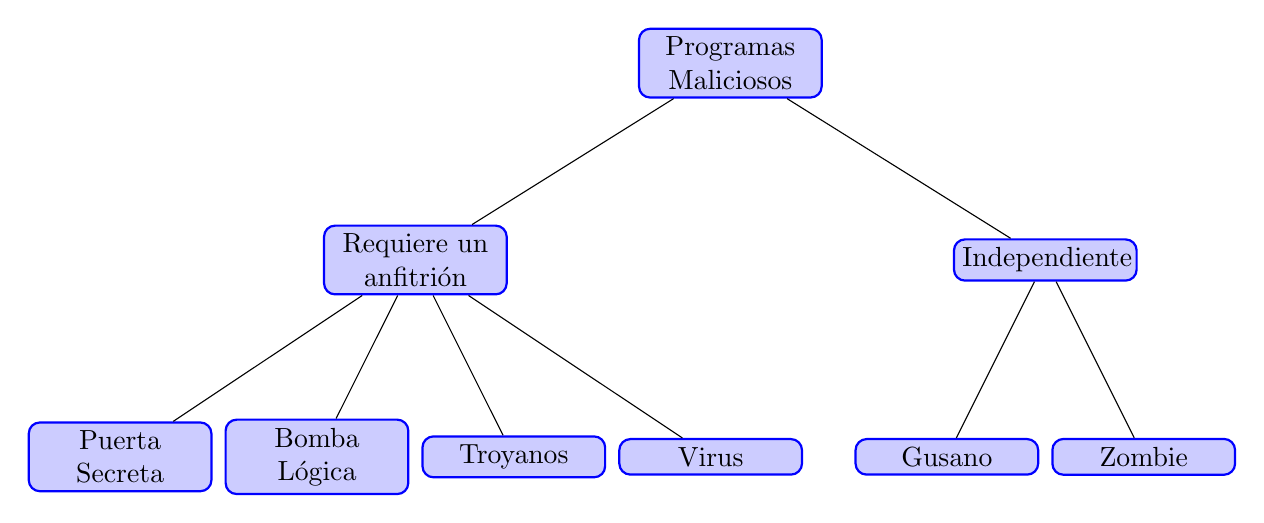
\begin{tikzpicture}[auto, every node/.style={draw=blue, thick, fill=blue!20,
                text width=6em, text badly centered,inner sep=3pt, rounded corners}, 
                 level 1/.style={sibling distance=80mm, level distance=2.5cm},
                 level 2/.style={sibling distance=25mm, level distance=2.5cm}]
        \node[draw](z){Programas Maliciosos}
            child{ 
                node {Requiere un anfitrión}
                child{
                    node {Puerta Secreta} }
                child{
                    node {Bomba Lógica} }
                child{
                    node {Troyanos} }
                child{
                    node {Virus} }
            }
            child{ 
                 node {Independiente}
                 child{
                     node {Gusano} }
                 child{
                     node {Zombie} }
        };
    \end{tikzpicture}
    \label{fig:malware}
\end{figure}

%%%%%%%%%%%%%%%%%%%%%%%%%%%%%%%%%%%%%%%%%%%%%%%%%%%%%%%%%%%%%%%%%%%%%%%%%%%%%% 
